% -*- root: apunte-metodos.tex -*-

\section{Ceros de funciones}

Como ya hemos visto, a la hora de resolver sistemas de ecuaciones lineales,
existe una gran variedad de métodos entre los cuales elegir. No obstante, si
bien las ecuaciones lineales permiten modelar, o al menos aproximar, una
inmensa cantidad de problemas, en muchas ocasiones se vuelve necesario
resolver ecuaciones que no son lineales. Si bien para algunos casos
particulares existen resoluciones analíticas, esto no es cierto en el caso
general; a modo de ejemplo, para los polinomios de grado cinco o superior,
es posible demostrar que no existen fórmulas algebraicas cerradas que permitan
obtener sus raíces. Esto hace que se trate de un problema complejo, y que
depende en gran medida de características particulares de la ecuación que se
busca resolver.

En general, una \textbf{ecuación} no (necesariamente) lineal \textbf{en una
variable real} es una expresión de la forma $f(x) = g(x)$, donde la variable
$x$ representa un valor desconocido. Para resolver la ecuación, se busca
para esta variable un valor $x^\ast \in \reals$ que satisfaga la igualdad.

Si definimos $h(x) = f(x) - g(x)$, lo que buscamos ahora es un valor $x^\ast$
satisfaga $h(x^\ast) = 0$, es decir, un \textbf{cero} de la función $h$.
A continuación, estudiaremos algunos métodos iterativos que permiten hallar
ceros de funciones en el caso general. Es decir, dada una función $f$,
buscaremos definir una sucesión
$\lbrace x_k \rbrace_{k \in \nats} \in \reals^\nats$ de modo que
$\lim_{k \to \infty} x_k = x^\ast$, con $f(x^\ast) = 0$.

\subsection{Orden de convergencia}

Sea $\lbrace x_k \rbrace_{k \in \nats}$ una sucesión tal que
$\lim_{k \to \infty} x_k = x^\ast$. Decimos que
$\lbrace x_k \rbrace_{k \in \nats}$ tiene \textbf{orden de convergencia} $p$
si
\[ \lim_{k \to \infty} \frac{\lvert x_{k+1} - x^\ast \rvert}
    {\left( \lvert x_k - x^\ast \rvert \right)^p} = c > 0. \]
Informalmente, esto se puede interpretar de la siguiente forma: tomando
valores suficientemente grandes de $k$, se cumple que
$\lvert x_{k+1} - x^\ast \rvert \approx c \cdot \left(\lvert x_k - x^\ast \rvert\right)^p$
para algún $c > 0$.

\begin{itemize}
\item Si $p = 1$, decimos que la convergencia es \textbf{lineal}.
\item Si $p = 2$, decimos que la convergencia es \textbf{cuadrática}.
\item Si $1 < p < 2$, decimos que la convergencia es \textbf{superlineal}.
\end{itemize}

El orden de convergencia nos permite estimar la velocidad con la que las
aproximaciones arrojadas por el método analizado convergen al valor buscado.
Un orden de convergencia más alto indica una convergencia más rápida.

% \begin{tikzpicture}
%     \begin{axis} [
%         grid=both,
%         samples=11,
%         width=12 cm,
%         height=8 cm,
%         % restrict y to domain=0.0000000000001:1,
%     ]
%         \addplot[smooth, only marks, mark=*, domain=0:10, color=violet] {(1/2)^x};
%         \addplot[smooth, only marks, mark=*, domain=0:10, color=teal] {(1/2)^(2^x-1)};
%     \end{axis}
% \end{tikzpicture}

Contamos además con el siguiente criterio para comparar el orden de
convergencia de dos sucesiones: sean $\lbrace \alpha_k \rbrace_{k \in \nats}$,
$\lbrace \beta_k \rbrace_{k \in \nats}$ dos sucesiones tales que
$\alpha_k \xrightarrow{k \to \infty} \alpha$ y
$\beta_k \xrightarrow{k \to \infty} 0$.
Si existe algún $k_0 \in \nats$ tal que, para todo $k \geq k_0$,
$\lvert \alpha_k - \alpha \rvert \leq \lvert \beta_k \rvert$,
entonces $\alpha_k$ se acerca a $\alpha$ al menos tan rápidamente como $\beta_k$
se acerca a $0$. En tal caso, si $\lbrace \beta_k \rbrace_{k \in \nats}$ tiene
orden de convergencia $p$, decimos que $\lbrace \alpha_k \rbrace_{k \in
\nats}$ tiene orden de convergencia al menos $p$.

\subsection{Criterios de parada}

Es necesario contar con un criterio que permita decidir cuándo la aproximación
ya es lo suficientemente buena, para así detener la ejecución del algoritmo.
Esto se conoce como \textbf{criterio de parada}. Algunos de los criterios más
comúnmente utilizados en algoritmos para la búsqueda de ceros de funciones
son:
\begin{enumerate}[label=(\roman*)]
\item Establecer una cantidad fija de iteraciones. Es el criterio más sencillo,
    pero es insensible a las características del método usado y no permite
    decidir \emph{a priori} la precisión de los resultados.
\item Fijar un valor $\varepsilon > 0$ y parar cuando
    $\lvert x_{k+1} - x_k \rvert < \varepsilon$, es decir, cuando el ritmo de
    convergencia sea lo suficientemente lento. Si bien es un criterio más
    sofisticado, puede dar resultados erróneos. Por ejemplo, considerando la
    sucesión $x_k = \sum_{i=0}^k \frac{1}{k} = 1 + \frac{1}{2} + \dots +
    \frac{1}{k}$, se tiene que $\lvert x_{k+1} - x_k \rvert = \frac{1}{k+1}
    \xrightarrow{k \to \infty} 0$. Luego, para cualquier valor de
    $\varepsilon$, el criterio terminará y arrojará un resultado
    supuestamente cercano al límite de la sucesión, que en realidad es
    divergente.
\item Fijar un valor $\varepsilon > 0$ y parar cuando
    $\frac{\lvert x_{k+1} - x_k \rvert}{\lvert x_k \rvert} < \varepsilon$. La
    idea, en este caso, es testear el error relativo de la aproximación.
    Sufre de problemas similares al criterio anterior, pero es un buen
    candidato a utilizar en la ausencia de información adicional.
\item Fijar un valor $\varepsilon > 0$ y parar cuando $f(x_k) < \varepsilon$.
    También puede dar falsos positivos, ya que $f$ puede tomar valores
    arbitrariamente cercanos a $0$ sin que esto indique la cercanía de una
    raíz.
\item Fijar un valor $\varepsilon > 0$ y parar cuando $\lvert f(x_{k+1}) -
    f(x_k) \rvert < \varepsilon$.
\item Fijar un valor $\varepsilon > 0$ y parar cuando $\frac{\lvert f(x_{k+1})
    - f(x_k) \rvert}{\lvert f(x_k)\rvert} < \varepsilon$.
\end{enumerate}

Como puede verse, todos estos criterios tienen casos patológicos en los que
arrojan resultados falsos. Por este motivo, la elección del criterio de parada
debe hacerse teniendo en cuenta las características del problema a resolver.
Además, es posible emplearlos de forma combinada; por ejemplo, es común
establecer un límite fijo de iteraciones incluso aunque se use un criterio de
parada distinto, para evitar la posibilidad de caer en un \emph{loop} infinito
si la sucesión diverge.

\subsection{Método de la bisección}

Consideremos una función continua $f : [a,b] \to \reals$ tal que $f(a) \cdot
f(b) < 0$; es decir, cuyos valores en los extremos tienen signos opuestos.
Entonces, por el teorema de Bolzano, la función tiene algún cero en el
intervalo $(a,b)$, es decir, existe $x^\ast \in (a,b)$ tal que $f(x^\ast) = 0$.

El \textbf{método de la bisección} permite, bajo dichas condiciones,
encontrar este valor $x^\ast$. La idea es similar a la búsqueda binaria: se
comienza por dividir el intervalo $(a,b)$ en dos mitades. Necesariamente
el valor $x^\ast$ buscado estará en una de estas mitades; se identifica de cuál
de las dos se trata, y se repite el procedimiento en el nuevo intervalo.
De esta forma, con cada iteración, se obtiene un intervalo de menor longitud
que contiene a la raíz buscada, lo cual permite aproximarla con precisión
arbitraria.

El pseudocódigo del algoritmo es el siguiente (debe ser completado con algún
criterio de parada).

\begin{algorithm}[H]
\caption{Algoritmo de la bisección}
\label{algo:biseccion}

\Input{$a, b \in \reals$, y $f : [a,b] \to \reals$ tal que
    $f(a) \cdot f(b) < 0$}
\Output{una aproximación de una raíz $x^\ast \in (a,b)$ de $f$}

$a_0 \gets a$ \;
$b_0 \gets b$ \;

\For {$k = 0,1,2,\dots$} {
    $c_k \gets \frac{a_k + b_k}{2}$ \;
    \If {$f(c_k) = 0$} {
        \Return $c_k$ \;
    }
    \eIf {$f(c_k) \cdot f(a_k) < 0$} {
        $a_{k+1} \gets a_k$ \;
        $b_{k+1} \gets c_k$ \;
    }
    {
        $a_{k+1} \gets c_k$ \;
        $b_{k+1} \gets b_k$ \;
    }
}

\end{algorithm}

Es claro que, en el método de la bisección, $c_k \xrightarrow{k \to \infty}
x^\ast$ con $f(x^\ast) = 0$. Más aún, para todo $k \in \nats$, tanto $x^\ast$
como $c_k$ pertenecen al intervalo $[a_{k+1}, b_{k+1}]$, y como la longitud de
estos intervalos se reduce a la mitad en cada iteración, tenemos que
\[ \lvert c_k - x^\ast \rvert \leq \lvert b_{k+1} - a_{k+1} \rvert =
    \left\lvert \frac{b - a}{2^{k+1}} \right\rvert \]
es decir, el método de la bisección converge a $x^\ast$ al menos tan
rápidamente como la sucesión $\left\lbrace \frac{b - a}{2^{k+1}}
\right\rbrace_{k \in \nats}$ converge a $0$. Esta última tiene un
orden de convergencia lineal, lo cual nos permite afirmar que el método de la
bisección se aproxima al menos linealmente a una raíz de $f$.

% \begin{tikzpicture}
%     \begin{axis} [
%         grid = both,
%     ]
%         \addplot[smooth, no marks] {x^2};
%     \end{axis}
% \end{tikzpicture}

\subsection{Algoritmos de punto fijo}

Dada una función $g : [a,b] \to \reals$, se llama \textbf{punto fijo} de $g$ a
un valor $p \in [a,b]$ tal que $g(p) = p$.

El problema de encontrar ceros de funciones está fuertemente relacionado con
la búsqueda de puntos fijos. En efecto, dada una función $f$, existen diversas
formas de definir una función $g$ de modo tal que las raíces de $f$ sean los
puntos fijos de $g$. Por ejemplo, para $\lambda \neq 0$, se puede definir la
función $g(x) = x + \lambda \cdot f(x)$. Así, para cualquier valor $x^\ast$,
\[ g(x^\ast) = \lambda \cdot f(x^\ast) + x^\ast = x^\ast
    \qquad \text{sii} \qquad f(x^\ast) = 0 \]
por lo que $x^\ast$ será un punto fijo de $g$ si y solo si es una raíz de $f$.

La ventaja de transformar el problema de esta manera radica en que existe una
idea sumamente sencilla que puede aplicarse para buscar los puntos fijos de
una función a través de un método iterativo. Considerando una función $g :
[a,b] \to \reals$ cualquiera y fijando algún punto inicial $x_0 \in [a,b]$, se
puede definir la sucesión $\lbrace x_k \rbrace_{k \in \nats}$ con
\[ x_{k+1} = g(x_k) \]
Si existe $\lim_{k \to \infty} x_k = x^\ast$, tomando límite de ambos lados en
la ecuación anterior, resulta que
\[ x^\ast = \lim_{k \to \infty} x_{k+1} = \lim_{k \to \infty} g(x_k) = g(x^\ast) \]
por lo que $x^\ast$ deberá ser un punto fijo de $g$.

Queda por determinar bajo qué condiciones es posible asegurar que este método
converge, y que lo hace en forma eficiente; a continuación se enuncian algunos
resultados que resultan útiles en este sentido. Sea una función $g: [a,b] \to
[a,b]$. Se cumplen:

\begin{enumerate}[label=(\roman*)]
\item Si $g$ es continua, entonces $g$ tiene al menos un punto fijo en $[a,b]$.

    % \emph{Demostración:}
    % Si $g(a) = a$ o $g(b) = b$, la afirmación es trivialmente verdadera. En
    % caso contrario, debe ser $g(a) > a$ y $g(b) < b$. Considerando
    % entonces la función continua $h(x) = g(x) - x$, tenemos que $h(a) > 0$ y
    % $h(b) < 0$. Aplicando el teorema de Bolzano, existe $p \in (a,b)$ tal que
    % $h(p) = 0$, y por lo tanto, $g(p) = p$.
\item Si, además, $g$ es derivable en $(a,b)$ y existe alguna constante $c$,
    con $0 < c < 1$, tal que
    $\fall{x \in (a,b)} \lvert g'(x) \rvert \leq c$,
    entonces el punto fijo es único.

    % \emph{Demostración:}
    % Sean $p_1, p_2 \in [a,b]$ puntos fijos de $g$. Supongamos $p_1 \neq
    % p_2$. Por el Teorema del Valor Medio, existe $\xi \in (a,b)$ tal que
    % $\lvert g'(\xi) \rvert
    % = \left\lvert \frac{g(p_1) - g(p_2)}{p_1 - p_2} \right\rvert
    % = \left\lvert \frac{p_1 - p_2}{p_1 - p_2} \right\rvert = 1$, lo cual
    % es absurdo, ya que $\fall{x \in (a,b)} \lvert g'(x) \rvert \leq k < 1$.
    % Debe ser, entonces, que $p_1 = p_2$.
\item Bajo estas condiciones, para cualquier $x_0 \in [a,b]$, la sucesión dada
    por $x_{k+1} = g(x_k)$ converge al único punto fijo de $g$ en $[a,b]$.

    % \emph{Demostración:}
    % Sabemos, por el Teorema del Valor Medio, que para todo $k \in \nats_{>0}$
    % existe un valor $\xi_k \in (a,b)$ tal que
    % \[ \lvert x_k - x^\ast \rvert = \lvert g(x_{k-1}) - g(x^\ast) \rvert =
    %     \lvert g'(\xi_k) \rvert \cdot \lvert x_{k-1} - x^\ast \rvert \leq
    %     c \cdot \lvert x_{k-1} - x^\ast \rvert \]
    % Aplicando sucesivas veces esta desigualdad, vemos que
    % \[ 0 \leq \lvert x_k - x^\ast \rvert
    %     \leq c \cdot \lvert x_{k-1} - x^\ast \rvert
    %     \leq c^2 \cdot \lvert x_{k-2} - x^\ast \rvert \leq \dots
    %     \leq c^k \cdot \lvert x_{0} - x^\ast \rvert \]
    % Como $0 < c < 1$, $c^k \xrightarrow{k \to \infty} 0$, y tomando límite,
    % obtenemos
    % \[ 0 \leq \lim_{k \to \infty} \lvert x_k - x^\ast \rvert
    %     \leq \lim_{k \to \infty} c^k \cdot \lvert x_{0} - x^\ast \rvert = 0 \]
    % de donde se sigue que $\lim_{k \to \infty} \lvert x_k - x^\ast \rvert = 0$,
    % es decir, $\lim_{k \to \infty} x_k = x^\ast$.
    \label{punto-fijo:cond-convergencia}
\end{enumerate}

En cuanto a la velocidad de convergencia, podemos afirmar que:

\begin{enumerate}[label=(\roman*),resume]
\item Bajo las hipótesis del punto \ref{punto-fijo:cond-convergencia}
    anterior (es decir, $g:[a,b] \to [a,b]$ continua, derivable en $(a,b)$,
    con $\lvert g'(x) \rvert \leq c < 1$ para algún valor $c$), pueden
    extraerse cotas que relacionan el error de aproximación cometido por el
    algoritmo en la iteración $k$-ésima con el valor de $c^k$. Esto permite
    deducir que, cuanto menor sea la cota que pueda imponerse a la derivada de
    la función $g$, más rápida será la convergencia garantizada por el
    algoritmo.

\item Si se tiene una función $g \in \mathcal{C}^r([a,b])$ (es decir, $g$ es
    $r$ veces derivable en $(a,b)$ con derivada continua) y un valor de $x_0$
    tales que la iteración $x_{k+1} = g(x_k)$ converge a un punto fijo $x^\ast
    \in (a,b)$, y se cumple que
    \begin{itemize}
    \item $g'(x^\ast) = g''(x^\ast) = \dots = g^{(r-1)}(x^\ast) = 0$, y
    \item $g^{(r)}(x^\ast) \neq 0$,
    \end{itemize}
    entonces el orden de convergencia de $\lbrace x_k \rbrace_{k \in \nats}$
    es $r$.
\end{enumerate}

A continuación, veremos cómo pueden aprovecharse estos resultados para
convertir el problema de hallar ceros de una función en un problema de punto
fijo, asegurando que la sucesión obtenida converge y que lo hace de manera
rápida.

\subsection{Método de Newton}

El \textbf{método de Newton} es un algoritmo para la búsqueda de raíces de
funciones, se basa en plantear una iteración de punto fijo que, bajo ciertas
hipótesis, converge con orden al menos cuadrático.

El método requiere que se considere una función $f \in \mathcal{C}^2([a,b])$, y que
podamos calcular los valores de $f$ y de su derivada. Se comienza con un valor
$x_0 \in ([a,b])$ y, en cada iteración, se utiliza la derivada de $f$ para aproximar el
comportamiento de $f$ en un entorno del valor actual y, de esa forma,
ir acercándose de manera iterativa a una raíz de la función.

En concreto, buscaremos un punto fijo de la función
\[ g(x) = x - \frac{f(x)}{f'(x)}, \]
con lo cual la iteración de punto fijo quedará definida por
\[ x_{k+1} = x_k - \frac{f(x_k)}{f'(x_k)}. \]

Si queremos utilizar el algoritmo para encontrar una raíz $x^\ast \in ([a,b])$ de $f$, será necesario que $g$ esté bien definida en un entorno de $x^\ast$, es decir, que $f'(x^\ast) \neq 0$. En ese caso, resulta que
\[ g(x^\ast) = x^\ast - \frac{f(x^\ast)}{f'(x^\ast)} = x^\ast, \]
es decir, $x^\ast$ es efectivamente un punto fijo de $g$.

Además, podemos notar que, en ese caso, se cumple que
\[ g'(x^\ast) = \frac{f(x^\ast) \cdot f''(x^\ast)}{f'(x^\ast)^2} = 0. \]
Como $g'$ es continua, existe un entorno $(x^\ast - \delta, x^\ast + \delta)$ de $x^\ast$ en el cual $\lvert g'(x) \rvert \leq c$ con $0 < c < 1$. Se puede demostrar que la restricción de $g : [x^\ast - \delta, x^\ast + \delta] \to [x^\ast - \delta, x^\ast + \delta]$ está bien definida. Teniendo en cuenta los resultados previos, esto nos permite afirmar que, en dicho entorno, el método converge a la raíz $x^\ast$ y lo hace con un orden de convergencia al menos cuadrático.

Cabe destacar que la convergencia solo puede asegurarse dentro de un entorno,
tal vez reducido, de $x^\ast$. Esto hace que el método solo funcione
correctamente si se parte de una aproximación más o menos buena de una raíz
de la función. Una solución común a este problema, cuando no se cuenta con
dicha aproximación, es obtenerla en primer lugar ejecutando algunas
iteraciones del método de la bisección.

El método tiene una interpretación geométrica muy intuitiva, que 
observarse en la Figura \ref{fig:newton}. Partiendo de un
punto $x_0$, se considera la recta tangente a $f$ en el
punto $(x_0, f(x_0))$. El punto $x_1$ se define como la intersección entre
esta recta y el eje de abscisas. El proceso se repite con cada iteración,
arrojando cada vez una aproximación más cercana a la raíz $x^{\ast}$
buscada.

\begin{figure}[H]
\centering
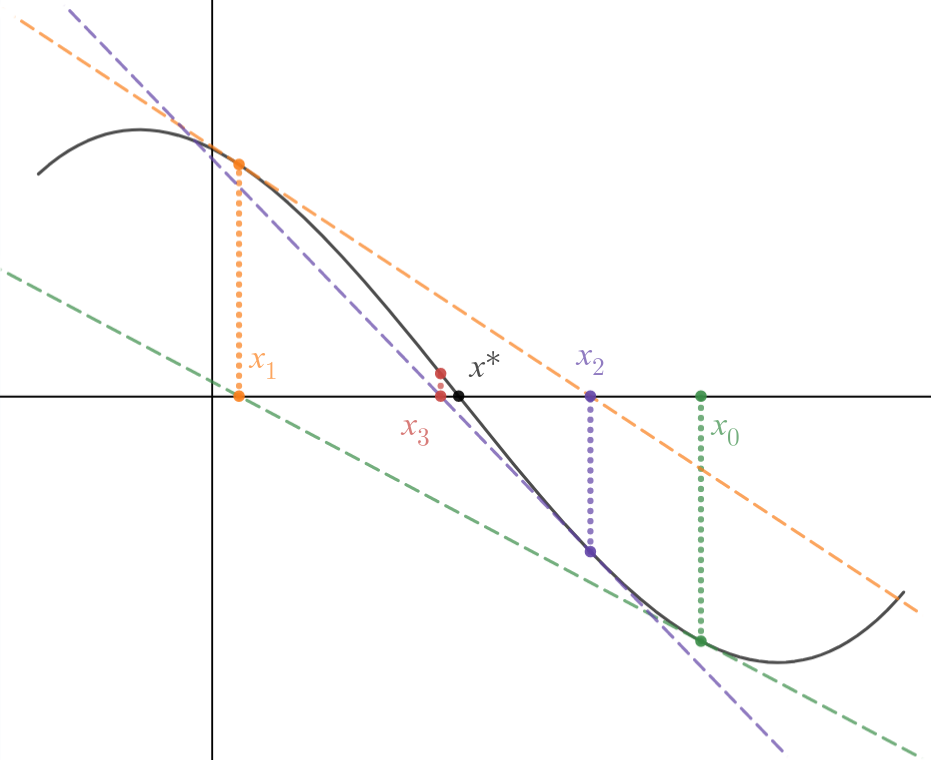
\includegraphics[width=10cm]{newton.png}
\caption{Interpretación geométrica del método de Newton.}
\label{fig:newton}
\end{figure}

Se trata de un método que, bajo las condiciones adecuadas, converge a una
buena velocidad. Sin embargo, tiene dos principales desventajas. Una de ellas
ya se mencionó anteriormente, y es la necesidad de conocer de antemano una
aproximación relativamente buena de la raíz buscada para poder asegurar la
convergencia; más aún si se desea que la convergencia sea rápida, ya que
el orden cuadrático puede resultar excesivamente lento si se comienza demasiado
lejos de la raíz. La otra desventaja es la necesidad de computar, en cada
paso, el valor de la derivada de $f$, lo cual puede ser difícil,
computacionalmente costoso o directamente imposible.

\subsection{Método de la secante}
El \textbf{método de la secante} es otra iteración de punto fijo que es
muy similar método de Newton, pero en lugar de considerar
la derivada de $f$ en el punto actual, la aproxima mediante la recta secante
que pasa por el punto actual y el punto anterior. Es decir, se considera que
\[ f'(x_k) \approx \frac{f(x_k) - f(x_{k-1})}{x_k - x_{k-1}}. \]

Como cada iteración tendrá en cuenta los dos puntos anteriores, se debe
comenzar determinando dos puntos iniciales, $x_0$ y $x_1$. Luego, la iteración
se define como
\[ x_{k+1} = x_k - \frac{f(x_k)}{\frac{f(x_k) - f(x_{k-1})}{x_k - x_{k-1}}}
           = x_k - \frac{f(x_k) \cdot (x_k - x_{k-1})}{f(x_k) - f(x_{k-1})}. \]

La Figura \ref{fig:secante} ilustra la interpretación geométrica de este
método.

\begin{figure}[H]
\centering
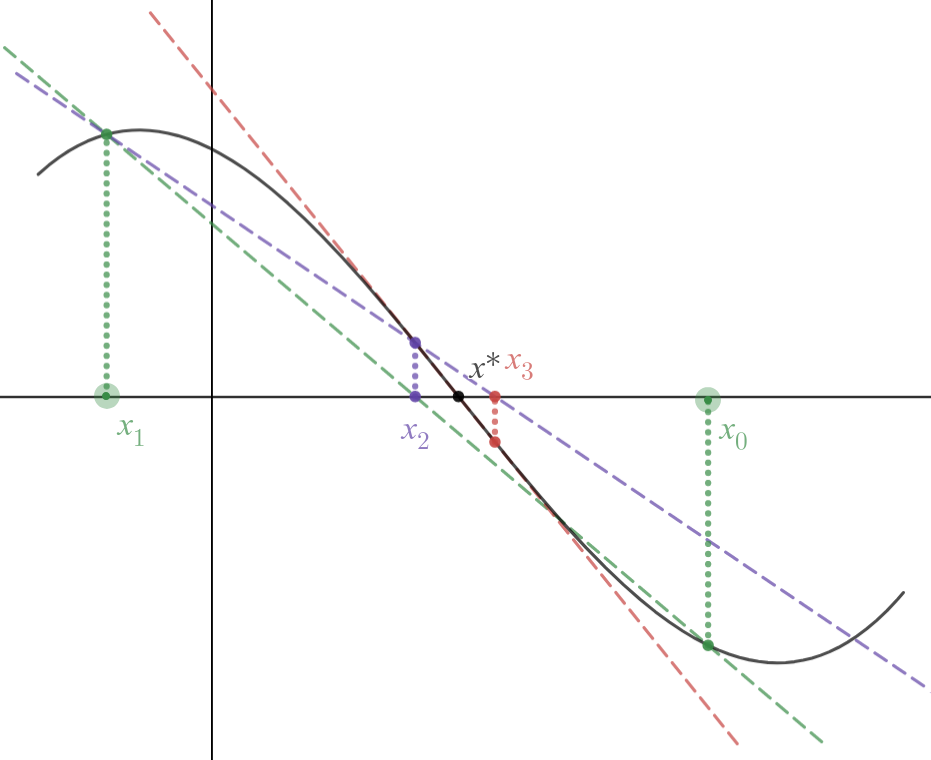
\includegraphics[width=10cm]{secante.png}
\caption{Interpretación geométrica del método de la secante.}
\label{fig:secante}
\end{figure}

El método de la secante converge un poco más lentamente que el método de
Newton. Sin embargo, puede demostrarse que su orden orden de convergencia es
supralineal: más exactamente, es $\varphi = \frac{1 + \sqrt{5}}{2}$, la
razón áurea. Además, presenta la gran ventaja de no requerir el cómputo
de ninguna derivada.

Uno de los inconvenientes que surge a la hora de utilizar este método tiene
que ver con la pérdida de dígitos significativos (o \emph{cancelación
catastrófica}) que se produce al tener que computar diferencias entre
valores que, con cada iteración, se encuentran cada vez más cerca; el método
\emph{regula falsi} presenta una alternativa que no padece de este problema.

\subsection{Método \emph{regula falsi}}
El \textbf{método \emph{regula falsi}} es una variante del método de
la bisección, que incorpora la idea principal del método de la secante.
Al igual que en el método de la bisección, se comienza con dos puntos
iniciales donde $f$ tiene distinto signo;
en cada paso se divide el intervalo en dos y se
pasa a trabajar con la parte en cuyos extremos $f$ tiene diferente signo.
Sin embargo, en lugar de dividir al intervalo por su punto medio, se utiliza
la intersección entre el eje de abscisas y la recta que pasa por los dos
puntos anteriores.

Este método converge con un orden lineal, de la misma forma que el método de
la bisección, pero resulta más rápido en términos prácticos. Comparado con
el método de la secante, si bien es más lento, reduce la posibilidad de que
se produzcan cancelaciones catastróficas: los valores de $f$ con los que
se trabaja siempre tienen signos opuestos, con lo cual las operaciones que se
realizan pueden pensarse como sumas en lugar de diferencias.
